\section{Rückgekoppelte Netze}
Neuronen sind beliebig miteinander verbunden, d.h. jedes Neuron kann mit jedem anderen Neuron verbunden sein. Die Kopplungsmatrix C hat keine spezielle Struktur.
\begin{figure}[h]
    \centering
    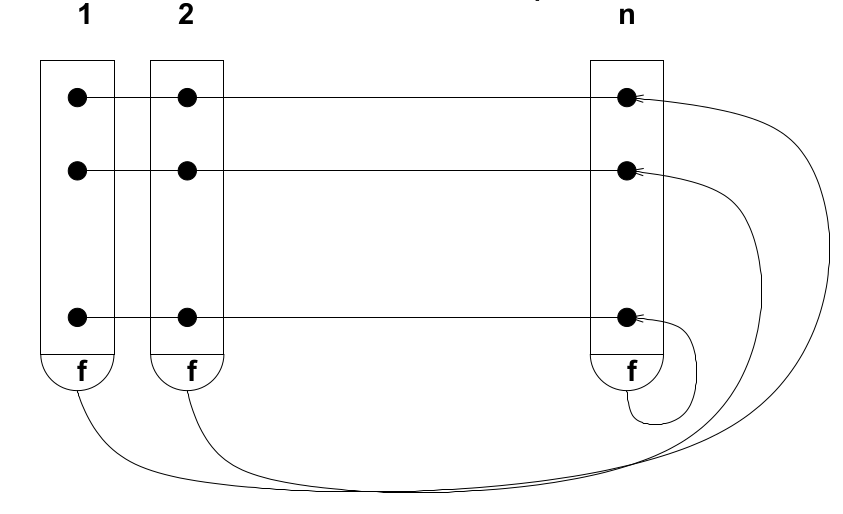
\includegraphics[width=0.25\textwidth]{img/NeuronaleArchitekturen/rueckgekoppelteNetze.png}
    \caption{Rückgekoppeltes Netz}
    \label{ch_arch_rueck}
\end{figure}

\section{Vorwärtsgekoppelte Netze}
\begin{itemize}
    \item Informationsfluss gerichtet: Eingabeneuron $\rightarrow$ Ausgabeneuron
    \item sequentielle Verarbeitung durch mehrere Neuronen/Schichten
    \item C ist durch eine Matrix gegeben $\rightarrow$ Graph zyklenfrei
\end{itemize}
Diese Art der Netze sind für die praktische Anwendung von großer Bedeutung.

\section{Geschichtete neuronale Netze}
\begin{itemize}
    \item Neuronen in Eingabeschicht geben Input nur weiter
    \item Neuronen in Schicht k: Input von k-1, Output an k+1 (hidden layer)
    \item letzte Schicht als Ausgabeschicht
\end{itemize}

\section{Darstellung von Mehrschicht-Netzen}
\begin{figure}[h]
    \centering
    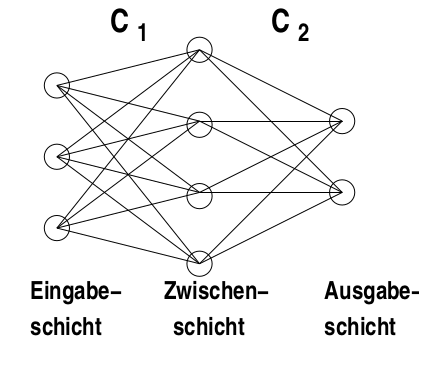
\includegraphics[width=.3\textwidth]{img/NeuronaleArchitekturen/d1.png}\hfill
    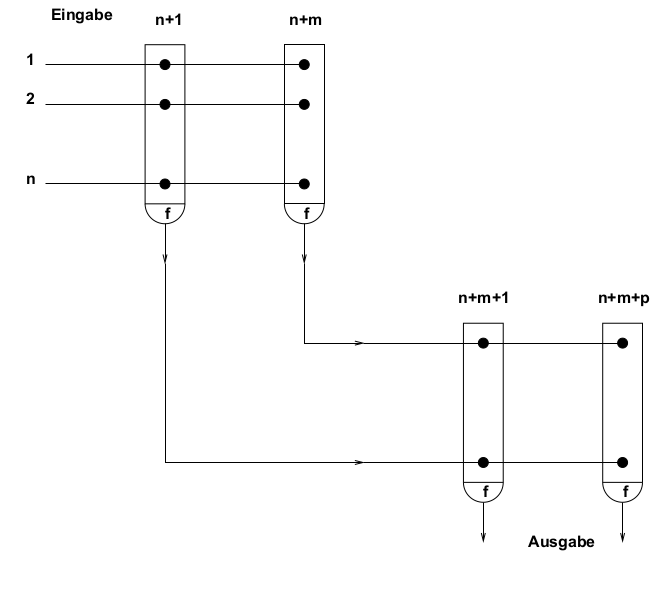
\includegraphics[width=.3\textwidth]{img/NeuronaleArchitekturen/d2.png}\hfill
    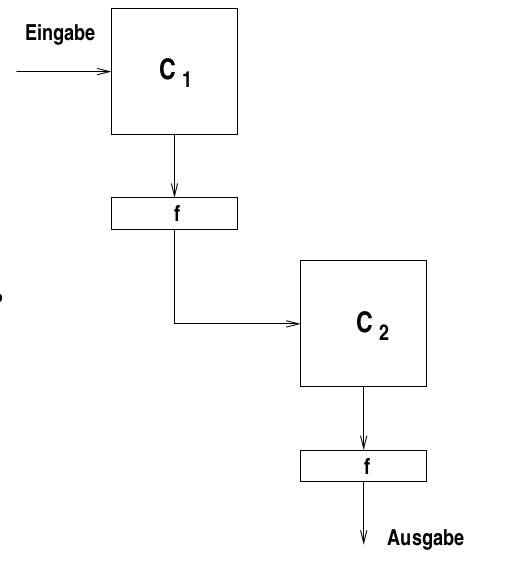
\includegraphics[width=.3\textwidth]{img/NeuronaleArchitekturen/d3.png}
    
    \caption{Darstellungsmöglichkeiten}
    \label{ch_arch_darst}
\end{figure}